%%%%%%%%%%%%%%%%%%%%%%%%%%%%%%%%%%%%%%%%%%%%%%%%%%%%%%%%%%%%
%%% LIVECOMS ARTICLE TEMPLATE FOR BEST PRACTICES GUIDE
%%% ADAPTED FROM ELIFE ARTICLE TEMPLATE (8/10/2017)
%%%%%%%%%%%%%%%%%%%%%%%%%%%%%%%%%%%%%%%%%%%%%%%%%%%%%%%%%%%%
%%% PREAMBLE
\documentclass[9pt,software]{livecoms}
% Use the 'onehalfspacing' option for 1.5 line spacing
% Use the 'doublespacing' option for 2.0 line spacing
% Use the 'lineno' option for adding line numbers.
% Use the "ASAPversion' option following article acceptance to add the DOI and relevant dates to the document footer.
% Use the 'pubversion' option for adding the citation and publication information to the document footer, when the LiveCoMS issue is finalized.
% The 'bestpractices' option for indicates that this is a best practices guide.
% Omit the bestpractices option to remove the marking as a LiveCoMS paper.
% Please note that these options may affect formatting.

\usepackage{lipsum} % Required to insert dummy text
\usepackage[version=4]{mhchem}
\usepackage{siunitx}
\DeclareSIUnit\Molar{M}
\usepackage[italic]{mathastext}
\graphicspath{{pictures/}}

%%%%%%%%%%%%%%%%%%%%%%%%%%%%%%%%%%%%%%%%%%%%%%%%%%%%%%%%%%%%
%%% IMPORTANT USER CONFIGURATION
%%%%%%%%%%%%%%%%%%%%%%%%%%%%%%%%%%%%%%%%%%%%%%%%%%%%%%%%%%%%

\newcommand{\versionnumber}{1.0}  % you should update the minor version number in preprints and major version number of submissions.
\newcommand{\githubrepository}{\url{https://github.com/thehamop1/AdvSoftwareEngineeringProject}}  %this should be the main github repository for this article

%%%%%%%%%%%%%%%%%%%%%%%%%%%%%%%%%%%%%%%%%%%%%%%%%%%%%%%%%%%%
%%% ARTICLE SETUP
%%%%%%%%%%%%%%%%%%%%%%%%%%%%%%%%%%%%%%%%%%%%%%%%%%%%%%%%%%%%
\title{Designing a scalable Conversational Interface}

\author[1\authfn{3}]{Cristian Gutierrez}
\author[1\authfn{3}]{Darshi Kasondra}
\author[1\authfn{3}]{Archana Ravi}
\author[1\authfn{3}]{Mounica Dingari}
\affil[1]{California State University of Northridge}

\corr{cristian.gutierrez.56@my.csun.edu}{CG}  % Correspondence emails.  FMS and FS are the appropriate authors initials.

\presentadd[\authfn{3}]{Department of Engineering and Computer Science, California State University of Northridge, United States of America}

\blurb{Additional work related to this paper can be fournd at \githubrepository;}

%%%%%%%%%%%%%%%%%%%%%%%%%%%%%%%%%%%%%%%%%%%%%%%%%%%%%%%%%%%%
%%% PUBLICATION INFORMATION
%%% Fill out these parameters when available
%%% These are used when the "pubversion" option is invoked
%%%%%%%%%%%%%%%%%%%%%%%%%%%%%%%%%%%%%%%%%%%%%%%%%%%%%%%%%%%%
\pubDOI{10.XXXX/YYYYYYY}
\pubvolume{<volume>}
\pubissue{<issue>}
\pubyear{<year>}
\articlenum{<number>}
\datereceived{Day Month Year}
\dateaccepted{Day Month Year}

%%%%%%%%%%%%%%%%%%%%%%%%%%%%%%%%%%%%%%%%%%%%%%%%%%%%%%%%%%%%
%%% ARTICLE START
%%%%%%%%%%%%%%%%%%%%%%%%%%%%%%%%%%%%%%%%%%%%%%%%%%%%%%%%%%%%

\begin{document}

\begin{frontmatter}
  \maketitle
  
  \begin{abstract}
    The way we use interact with systems is contantly evolving with new advances in technology. As buisness continue to need flexible user
    interfaces many of them are implementing conversatinal interfaces in order to fufill customer needs without having to require users
    to learn how to use an entirely seperate application in order to make transactions. Modern conversatinal interfaces are fairly powerful 
    with recent adavancements in natural language processing, integration with mobile asistants, and flexible frameworks. In this paper we 
    provide background to some of the concepts of conversatinal interfaces, examing the current state of commercially available
    solutions, and provide a reference architecture for implementing a system centered around a conversatinal interface.
  \end{abstract}
  
\end{frontmatter}

\section{Introduction}

\subsection{Previous Work}
The first chatbot named ELIZA was invented in 1966.The ability of the chatbot to communicate with the user was limited as it did not have enough knowledge. PARRY was invented in 1977 with improved features from ELIZA. PARRY also had limitations as it could not learn from the conversations and had low responding speed. Many chatbots were invented after that. All had some limitation either understanding the conversation or had low responding speed. ALICE was invented in 1995 based on the ELIZA. It worked on the pattern-matching algorithm but still had limitations as it did not have intelligent features. Later in the 20th century when Artificial Intelligence started to grow chatbots like Siri and Watson had better understanding and recognizing capabilities than the previous ones. Now, we are looking to make our chatbots more smarter by making it recognize different accents.

\subsection{Current Work}
With the recent surge of machine learning algorithms we now have a way of saving conversational context, Matching user responses not hardcoded into the system and can provide unique responses with generative models. Pattern matching is still often used in these new technologies as a fall back mechanism.When both machine learning and pattern matching are used if the confidence score of either algorithm is higher that intent is chosen. 

\subsection{Background}
There are some basic concepts that are universal to most conversatinal interface platforms. The first is the user utterance which can either come in 
the form of a text entry or speech with the use of a microphone. Additional signal processing is required to transcribe the audio signals into text. 
This text is usually normalized where all text has its puntuation removed and all letters are moved into the same letter case. Next depending on the 
platform various machine learning algorithms are used in order to extract certain key tokens from the string. The most intent which is the objective
of the user. For example the utterance "What is the weather in Los Angeles" would have the intenet of weather. This is a topic that the application
would have to be designed to respond to. Next would be entities which are certain tokens the application will use to complete requests once an intenet
has been deduced.

\section{Reference Architecture}
\subsection{Types Of Bots}
A somewhat theoretical definition for the types of CI/bots:                      
Dialogic Agent: This is something that understands the user and generates appropriate responses. 
Rational Agent :This type of bot must understand the user and also retrieve data from an external source of knowledge often referred to as a corpora of data. In a business context this could be a database or an external API.
Embodied Agent :This type of agent is the final extension of the first two. It not only understands the user and can provide relevant data back to the user but it can also be perceived as human-like by the user. The first chat bots (which were rule based) were even given names in order to create this illusion. Today in the UX design of conversational interfaces the concept of a persona still exists. Think of the voices you can select in personal assistants.

We have referenced two architectures in this paper : 
\begin{itemize}
  \item Azure architecture framework
  \item Using AWS
\end{itemize}

The generic architecture of conversational bots:
\begin{figure}
  \caption{ The architecture of conversational bot}
  \centering
  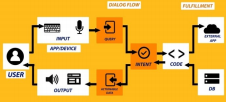
\includegraphics[width=0.5\textwidth]{simpleRef.png}
\end{figure}

In recent years, serverless architectures (Functions - as-a-Service) are gaining traction as an alternative way  of providing backend services without requiring a  dedicated infrastructure. Serverless allows its users to  deploy their stateless functions into platform  infrastructures. This stateless behavior makes every  invocation independent of the previous runs. For our  application, Firebase Cloud Functions and Google  Cloud Platform as our backend infrastructure is  provided.

\subsection{Azure architecture framework}

We used this as our reference architecture as it was easy for us to use the built in functions from Microsoft when trying to build the bot. The major components of this bot include

\begin{itemize}
  \item Bot logic and UX 
  \item Bot cognition and intelligence 
  \item Data ingestion and logging 
  \item Monitoring 
  \item Security and governance 
  \item Quality assurance and enhancements 
\end{itemize}

\begin{figure}
  \caption{Representation of the bot brain and the body}
  \centering
  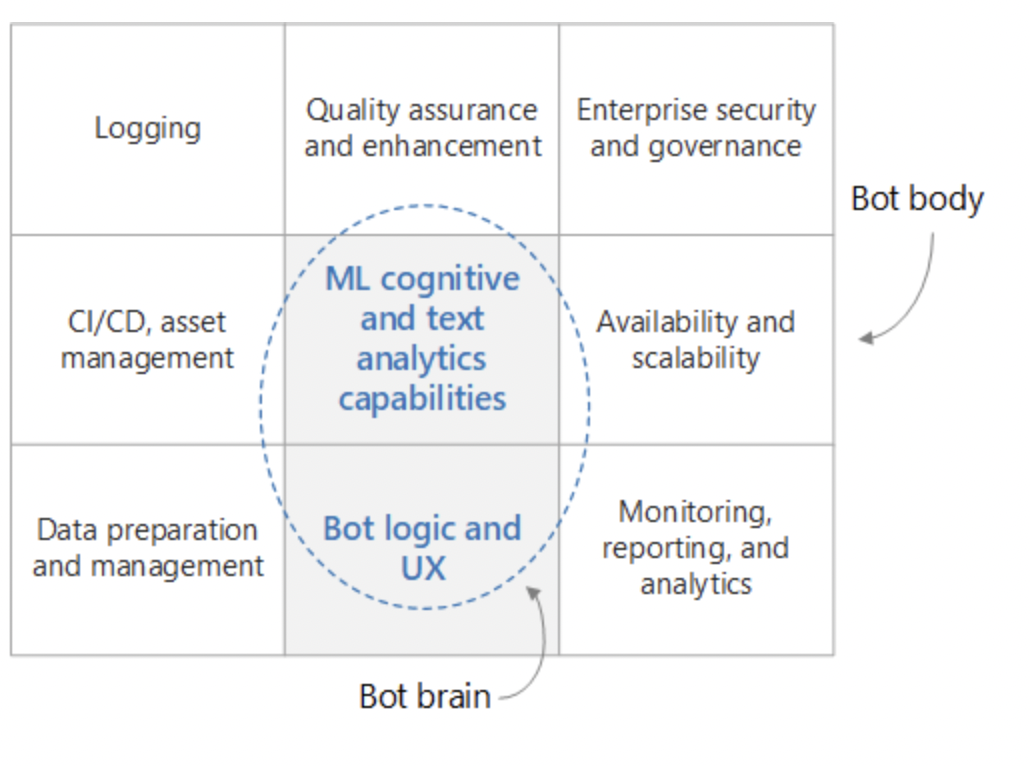
\includegraphics[width=0.5\textwidth]{table.png}
\end{figure}


1) Bot logic and user experience
Bot Framework Service (BFS). This service connects your bot to a communication app such as Cortana, Facebook Messenger, or Slack. It facilitates communication between your bot and the user.
Azure App Service. The bot application logic is hosted in Azure App Service.

2) Bot cognition and intelligence
Language Understanding (LUIS). Part of Azure Cognitive Services, LUIS enables your bot to understand natural language by identifying user intents and entities.
Azure Search. Search is a managed service that provides a quick searchable document index.
QnA Maker. QnA Maker is a cloud-based API service that creates a conversational, question-and-answer layer over your data. Typically, it's loaded with semi-structured content such as FAQs. Use it to create a knowledge base for answering natural-language questions.
Web app. If your bot needs AI solutions not provided by an existing service, you can implement your own custom AI and host it as a web app. This provides a web endpoint for your bot to call.

3)Data ingestion
The bot will rely on raw data that must be ingested and prepared. Consider any of the following options to orchestrate this process:
Azure Data Factory. Data Factory orchestrates and automates data movement and data transformation.
Logic Apps. Logic Apps is a serverless platform for building workflows that integrate applications, data, and services. Logic Apps provides data connectors for many applications, including Office 365.
Azure Functions. You can use Azure Functions to write custom serverless code that is invoked by a trigger — for example, whenever a document is added to blob storage or Cosmos DB.

4)Logging and monitoring
Application Insights. Use Application Insights to log the bot's application metrics for monitoring, diagnostic, and analytical purposes.
Azure Blob Storage. Blob storage is optimized for storing massive amounts of unstructured data.
Cosmos DB. Cosmos DB is well-suited for storing semi-structured log data such as conversations.
Power BI. Use Power BI to create monitoring dashboards for your bot.

5) Security and governance
Azure Active Directory (Azure AD). Users will authenticate through an identity provider such as Azure AD. The Bot Service handles the authentication flow and OAuth token management. See Add authentication to your bot via Azure Bot Service.
Azure Key Vault. Store credentials and other secrets using Key Vault.

6)Quality assurance and enhancements
Azure DevOps. Provides many services for app management, including source control, building, testing, deployment, and project tracking.
VS Code A lightweight code editor for app development. You can use any other IDE with similar features.


\begin{figure}
  \caption{Reference architecture using Azure inbuilt services}
  \centering
  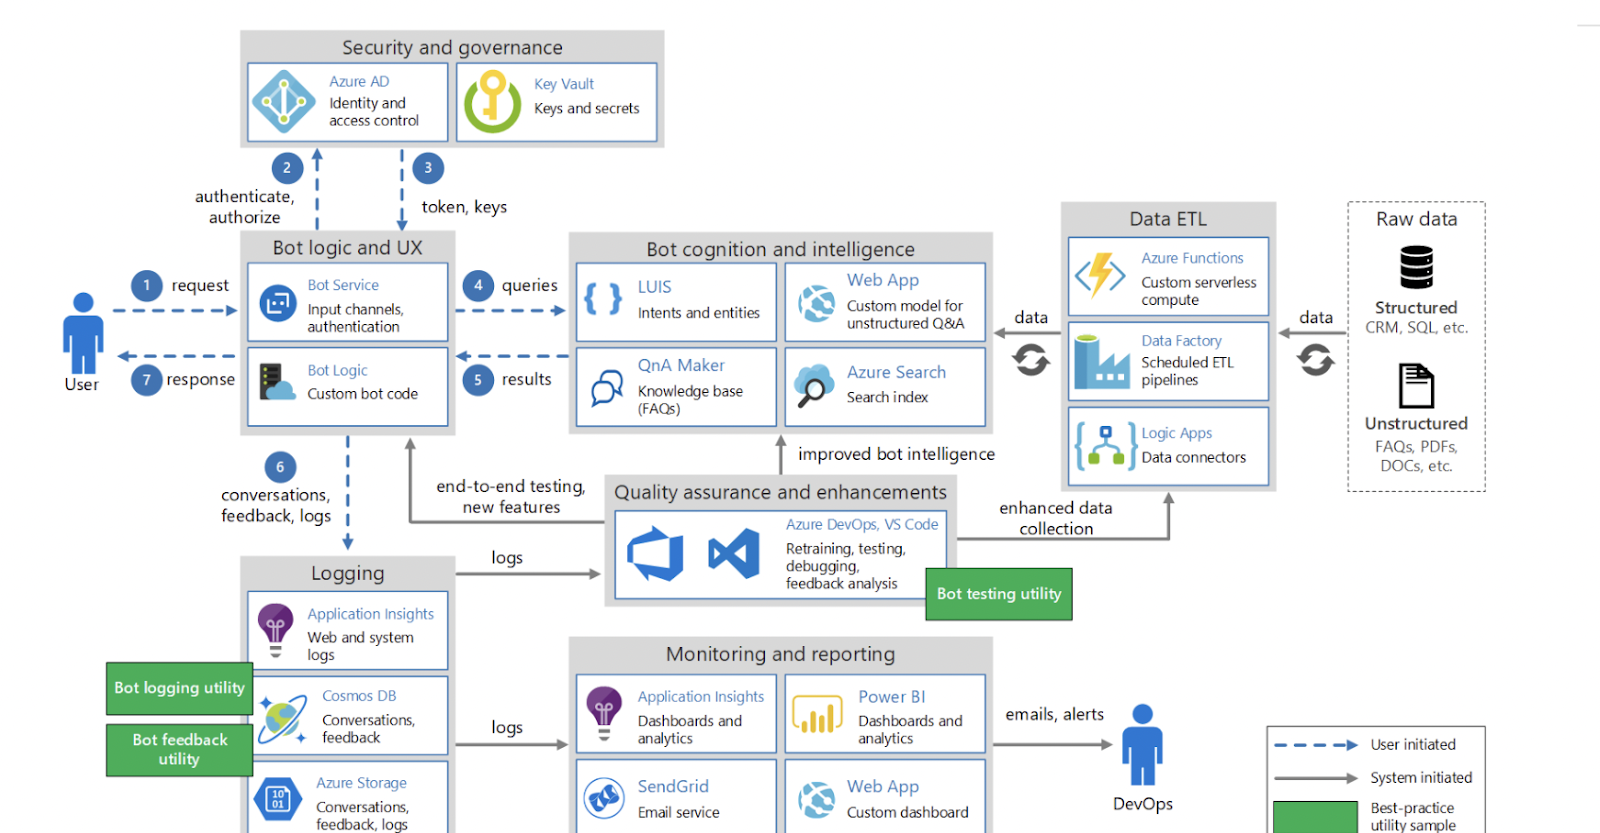
\includegraphics[width=0.5\textwidth]{azure.png}
\end{figure}

Now, Talking about Amazon Web Service Architecture, a Platform for computing at mobile edge. 
The architecture was broken down focusing on three major areas:
\subsection{Edge}
\begin{itemize}
\item Bringing data processing and analysis closer to end-points
\item Most extensive global cloud infrastructure
\item Build more quickly and reduce costs
\end{itemize}

\subsection{Cloud}
\subsection{Enterprise applications}



\section{Implementation Guide 1}
Chatbots have become a trending topic for organizations. It seems, marketing and artificial intelligence will be great allies in the next few years, while conversational commerce will play in favor of sales teams and social customer care, as well as resource optimization, it will also have significant returns for those in charge of operations. However, you must take into account some recommendations before implementing a chatbot.
83 percent of respondents in Deloitte’s State of AI Survey said they have achieved moderate or substantial benefits from their work with AI technologies, and 94 percent said AI is very or critically important to their success.
However, organizations still have plenty to learn about using chatbots in customer support and services scenarios, experts told CMSWire. And they're still making mistakes with such implementations. “One common mistake is many organizations start with ‘proof-of-concepts’ that are designed poorly and fail to support a company’s business objectives,” said Derek Top, research director and senior analyst for Opus Research. “Many firms underestimate the resources and staff necessary to provide a successful chatbot implementation.”
\subsection{Ensuring Accuracy of Chatbot Engine}
A company’s first-order concern should revolve around the accuracy of the chatbot “engine,” meaning its ability to correctly recognize end-user intents consistently and at sufficient scale. For many companies, accuracy is a moving target and highly-dependent on how much the data they have to ingest in the form of chat transcripts and other conversations. Contact centers are on the hook to manage a growing number of service channels, and chatbots are becoming a first-tier support option for helping augment the live support and drive efficiencies in the contact center. The goal is to engage customers, when appropriate, to support and answer user questions and take action to decrease costs and optimize service channels.

\subsection{Determining User Needs, Bot Channels}
Not having a clear goal for the chatbot design leads to an incorrect intent detection, so the bot ends up getting confused and the accuracy the bot has on solving queries drops significantly. Another widespread mistake is not deploying the bot to the proper channels.

\subsection{Purpose, Scripts and Flow}
Implementing a chatbot entails three steps: Establish the purpose, build the scripts and build the flow. All these must be aligned to a set of KPIs that will measure the performance of our chatbot. We need to define what a user will be able to do and what is going to be left out of the scope. We must understand which business cases are more reasonable to have an assistant for. We must empathize with how the assistant will be invoked by users, in what channels it makes sense for the app or skill to be available. As for flow, that’s when implementation turns to Natural Language Processing (NLP) and session management. Determine and build the required end points on your backend to fulfill the requests of our users. Write down behind-the-scenes decisions the system logic will have to make and finally build test cases and a test plan. Chatbots require specific skills for testing and during testing and new scenarios may arise that should feed the design process or even retrain our NLP model. While building the bot you must add all the necessary data capture points that will guarantee you are collecting the information needed to keep track of the KPIs you defined. Not having the proper metrics could lead to customer dissatisfaction and disengagement.

\subsection{Define the Type of Chatbot You Need}
Once the line of business and the real needs of each area have been defined, It’s time to define priorities. Possibly a chatbot can support you with more than one activity but, it is important to prioritize and understand the central function of the chatbot:

\subsection{Chatbots Are a Retrieval Mechanism}
The bottom line is that a customer support chatbot is an information retrieval mechanism. Search is a retrieval mechanism and an intelligent virtual assistant is a retrieval mechanism. And at the end of the day you need some mechanism that says, 'Tell me what you're looking for, or give me a signal.' And the signal is the intent, but the intent can also be enriched by other signals.”
And it isn’t easy work. "There's a lot of work in refactoring the content," Earley said, "and building the right information architecture and right content... You have to use knowledge engineering approaches.”


\begin{itemize}
\item Sale of products
\item Customer Support
\item News Sharing
\end{itemize}

It is possible to have a hybrid, for example, if among the priorities is improving customer service and to enable new sales channels, you can build a system capable of receiving customer service and making sales, but the evolution must be gradual. First developing the functions that will allow you to cover the needs according to the score and subsequently begin integrating more elements. 

\subsection{Chatbots Are a Retrieval Mechanism}
The bottom line is that a customer support chatbot is an information retrieval mechanism. Search is a retrieval mechanism and an intelligent virtual assistant is a retrieval mechanism. And at the end of the day you need some mechanism that says, 'Tell me what you're looking for, or give me a signal.' And the signal is the intent, but the intent can also be enriched by other signals.” And it isn’t easy work. "There's a lot of work in refactoring the content," Earley said, "and building the right information architecture and right content... You have to use knowledge engineering approaches.”


\section{Implementation Guide 2}

\subsection{Use Cases}
The following implementation guide was designed with the assumption that it would be used in a buisness context such as 
e-commerce site, resturant, or customer support. Additionally little sensitive information would be transmitted between the 
conversatinal interface and the service could be an addition to existing buisness infrastructure. Additionally this 
Implementation guide is more suitable for small to medium sized buisness who are looking to provide the user with 
the ability to retrieve basic data and transactions. Refer to Figure 1 for a reference architecture for this guide (The seperation of logic
should be similar however the frameworks themeselves have been switched in order to support Google DialogFlow V2/V3).

An example use case for this reference architecture would be a small chain of resturants. In this scenario a customer may
want to make reservations for instance while the resturant is closed. In this scenario integrating a conversatinal interface 
on the buisnesses website and mobile assistant would provide the user with the ability to create or cancel reservations while 
the buisness is currently closed. Even customers with little knowledge of how to browse the internet or create reservations online
would be able to interact with their mobile asistants in order to interact with the system.  

\subsection{Technical Stack}
For this particular implementation guide a stack such as ReactJs, SQL, nodejs, dialogflow, and Google Assistant/Siri would be used. NodeJS would
be used on the lambda functions and buisness enterprise. Any in buisness databases would be created with an SQL flavor and an ORM such as 
knex.js would be used to store various information. If a buisness did not have an existing website it would be created in ReactJS, alternatively 
if an existing website was already available a simple iframe based solution could be used from the existing dialogflow API integrations.

As stated before any interaction needed with existing buisness infrastructure could be handled with lambda funcitons. The existing language most 
supported by the Dialogflow API is NodeJS. It is extermly cost effective and easy to integrate using Google Cloud Functions. In order to fully take
advantage of deploying to various platforms different buisness logic needs to created to interact with various front-ends. The Dialogflow API allows
you to create specific reponses based on the clients platform in order not to overwhelm the client with long responses or provide more relevant information
to the user.  

An added benefit to using lambda functions is that all of the heavy machine learning processing is carried out on the Dialogflow API side so no heavy
processing is required within the runtime of the lambda itself. This allows the call from the client to be quickly parsed via a RESTful API call and 
intenets, entities, and context can already be deduced ahead of time. By allowing the buisness logic to be compeltley free of all machine learning it allows
the particular buisness implemnting the system save money on renting a fully dedicated server to run the machine learning algorithm. Keep in mind that although
the use of lambda functions reduces cost there is an additonal cost required for every call to the Dialogflow service. Additionally the version of the DialogFlow API 
used also factors into cost. If the complexity of the conversations are relativley simple version 2 of the API can be used to increase savings on this implementation.

The Dialogflow dashboard would need to be trained using a set of sample training data. Most of the internal machine learning algorithms are abstracted on this platform. 
What this means for the buisness trying to develop their platform with this tool is that the develop who they chose to hire doesnt need an extensive background in machine
learning in order to get things working in the first place. In addition to this sample training data simple regular expressions would be given to the DialogFlow agent in order
to fall back on when confidence scores get too low. 

Lastly in terms of getting a voice enabled conversatinal interface for this systmem would require the use of the newer DialogFlow V3 API or the use of a deprecated 
API in order to interface wtih the older DialogFlow version 2. Although this option is available using the newer nodejs package it is highly discouraged as this part
of the library is no longer receiveing updates. Additionally in order to connect this service to iOS an additionial layer of buisness logic has to be placed between the 
dialogflow API calls and the Siri front-end. The buisness should consider the development cost required in order to keep iOS integration supported versus how 
benefical it is from a buisness stand-point to keep it supported. 

\subsection{Cost Benefit Analysis}
In order to understand the on-going cost of having lambda function costs and DialogFlow API calls the following charts should be considered when 
considering the benefit of adding a converstaional interface to an e-commerce site. 

\begin{figure}
  \caption{DialogFlow Version 2}
  \centering
  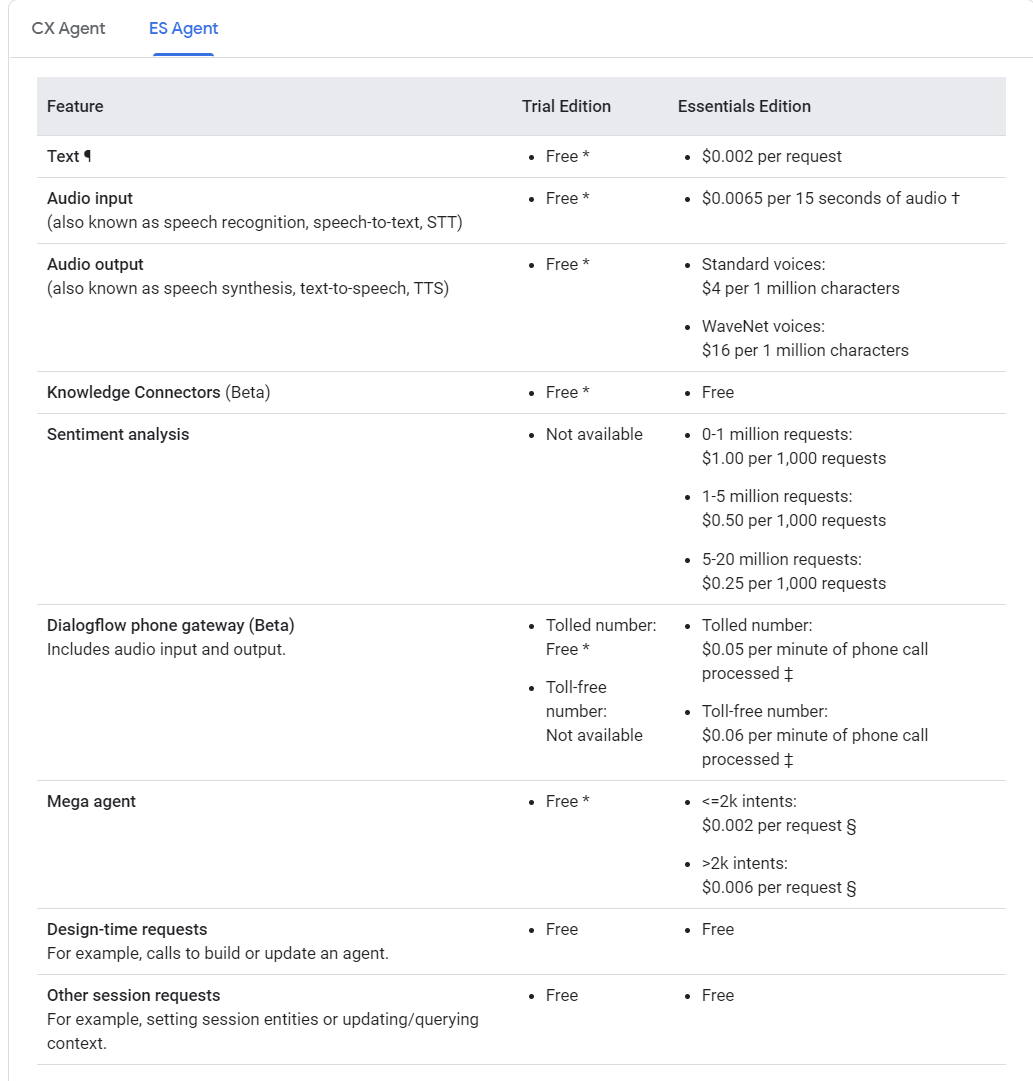
\includegraphics[width=0.5\textwidth]{ESAgent.PNG}
\end{figure}

\begin{figure}
  \caption{DialogFlow Version 3}
  \centering
  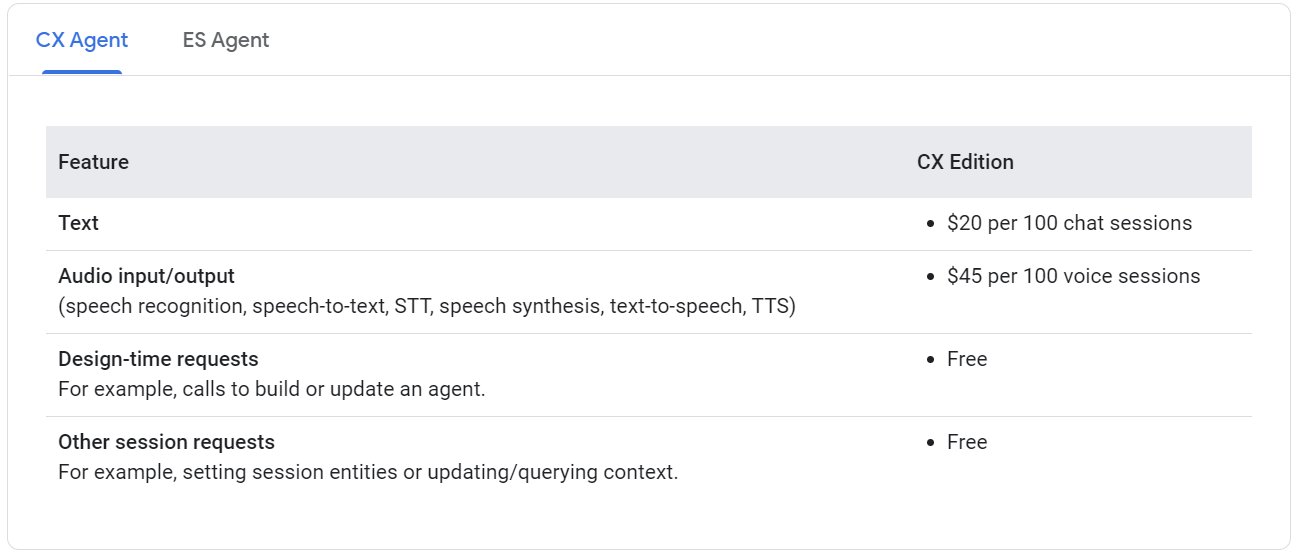
\includegraphics[width=0.5\textwidth]{CX_Agent.PNG}
\end{figure}

As seen above the cost of supporting the converstational interface API version 3 is far different that supporting version 2. If the buisness needs don't demand strict requirements 
that users will be generating complex utterances then version 2 of the API should be considered. If integration with google assistant and siri is an important feature then it's recommended
that Google Actions API be used (DialogFlow v3). Additionally the price of Google Cloud Function calls should also be considered. This service has a much lower cost especially if compute times
are kept low. See Figure 3.

\begin{figure}
  \caption{Google Cloud Function Pricing}
  \centering
  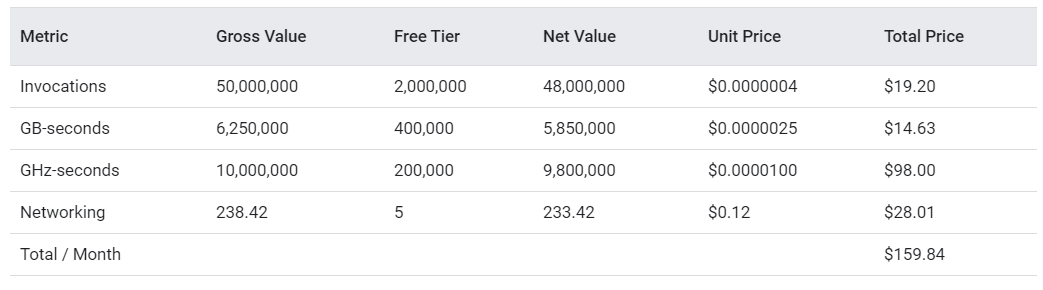
\includegraphics[width=0.5\textwidth]{GCloudFunction.PNG}
\end{figure}

\section{Development Plan}
\subsection{Configuration Management}
Within the Google Cloud Function dashboard a repository should be connected as the main source code for the lambda functions that will be servicing DialogFlow requests. This repository should be configured
with either the Github Flow or Git Flow configuration style. That being said in order to prevent disastrous situation such as a novice developer pushing to the deployment branch Continous Integration should
be implemented in order to verify that the deployed source code will work in production. Google Cloud can be configured in such a way most of the source conrol lives in Github or Bitbucket where the git server
can be configured to interact with Jenkins CI or Travis CI. Upon certain actions such as merging to the master the repository can automatically launch the newest source code
to the active lambdas.

\subsection{Development Environment}
Developers should use an environment where the same version of Node.JS that the Cloud Functions will be using. The appropriate version of DialogFlow for Node.js should be installed along with firebase lambda emulator.
This package allows developers to locally host a Google Cloud Function. Either ngrok or a similar package should be used in order to provide an https public facing URL in order to test with the DialogFlow 
agent via the DialogFlow dashboard. Additionally each developer should be given his/her own dashboard in order to connect their publically facing URL and test their code.

\section{Conclusion}
\subsection{Implementation}
In order to test our design while being platform agnostic the proposed objective was to create a DialogFlow agent that would interact with Github's RESTful API. Basic function available to the user would be searching
repositories, querying the git database for logs, merges, and pull requests. The front-end user interfaces would interact with the DialogFlow agent directly and once all necessary entities were detected the dialogflow agent
would make a request to the Web hook via Google Cloud Function (lambda function). The available front-ends deployed where integrations with Slack, basic web based GUI, and directly from the dashboard. The development enviroment 
consisted of Visual Studio Code, ngrok, firebase emulator, and the dialogflow test dashboard. A Git repository containing the DialogFlow fufillment code was hosted on Google Cloud where the master branch was set to deploy its newest commit.

\subsection{Challenges}
Several challenges were faced while implementting this conversrational interface. For example the dialogflow version 2 API was deprecated and full documentation to interact with the agent was no longer provided. Additionally in order to migrate
an existing workspace from DialogFlow V2 to Google Actions (v3) a length process needed to be followed in order to verify that the paths that the converstation could follow were correct. Additonally learning how to debug lambda functions on localhost 
was also a challenge there was sparse docuemntation from Google on how to accomplish this. 

\subsection{A Better Approach}
A better approach to this type of approach to this problem would be to implement directly with google actions and using ngrok and firebase emulator. By using Google Actions (V3 API) integration with mobile assistants becomes far 
easier and libraries have far better documenation and support from Google.

\subsection{Future Suggestions}
An extension to this simple implemenation is to create basic tests for the conversational interface. This would be useful for when conversations become much more complex and have to 
maintain contexts in order to give appropriate responses. Additionally creating a modular design to the fullfillment code would ensure that any future feature would be easy to integrate.


\bibliography{livecomsm-template-softwareanalyses}

\end{document}
